%%%%%%%%%%%%%%%%%%%%%%%%%%%%%%%%%%%%%%%%%%%%%%%%%%%%%%%%%%%%%%%%%%%%%%%%%%%%%%%%
%2345678901234567890123456789012345678901234567890123456789012345678901234567890
%        1         2         3         4         5         6         7         8

\documentclass[letterpaper, 10 pt, conference]{ieeeconf}  % Comment this line out if you need a4paper

%\documentclass[a4paper, 10pt, conference]{ieeeconf}      % Use this line for a4 paper

\IEEEoverridecommandlockouts                              % This command is only needed if 
                                                          % you want to use the \thanks command

\overrideIEEEmargins                                      % Needed to meet printer requirements.

%In case you encounter the following error:
%Error 1010 The PDF file may be corrupt (unable to open PDF file) OR
%Error 1000 An error occurred while parsing a contents stream. Unable to analyze the PDF file.
%This is a known problem with pdfLaTeX conversion filter. The file cannot be opened with acrobat reader
%Please use one of the alternatives below to circumvent this error by uncommenting one or the other
%\pdfobjcompresslevel=0
%\pdfminorversion=4

% See the \addtolength command later in the file to balance the column lengths
% on the last page of the document

% The following packages can be found on http:\\www.ctan.org
\usepackage{graphics} % for pdf, bitmapped graphics files
\usepackage{epsfig} % for postscript graphics files
%\usepackage{mathptmx} % assumes new font selection scheme installed
%\usepackage{times} % assumes new font selection scheme installed
\usepackage{amsmath} % assumes amsmath package installed
\usepackage{amssymb}  % assumes amsmath package installed

\title{\LARGE \bf
Comparison of Model-Based and Model-Free Reinforcement Learning and Optimal Control
}


\author{Julia Str\"obel, Sebastian H\"ugler, and Jan Br\"udigam}


\begin{document}



\maketitle
\thispagestyle{empty}
\pagestyle{empty}


%%%%%%%%%%%%%%%%%%%%%%%%%%%%%%%%%%%%%%%%%%%%%%%%%%%%%%%%%%%%%%%%%%%%%%%%%%%%%%%%
\begin{abstract}

The control of dynamical systems can be achieved by a variety of approaches with different advantages and drawbacks. In this paper, implementations of model-based reinforcement learning (RL), model-free RL, and optimal control for linear and non-linear dynamical systems are compared and discussed. The results show +one sentence about what results show+

\end{abstract}


%%%%%%%%%%%%%%%%%%%%%%%%%%%%%%%%%%%%%%%%%%%%%%%%%%%%%%%%%%%%%%%%%%%%%%%%%%%%%%%%
\section{INTRODUCTION}

The increase of computational power in recent years has allowed for the successful implementation of learning algorithms to control a wide range of dynamical systems. Nonetheless, classical approaches to control problems also provide 
useful solutions for this class of systems. Therefore, the aim of this paper is to present and discuss algorithms and results, as well as advantages and drawbacks of different control approaches, namely model-based reinforcement learning (RL), model-free RL, and optimal control. These methods are applied to a spring-mass system, a pendulum, and a cart-pole system.

The algorithms and results for the three approaches are presented in Sec. II, Sec. III, and Sec. IV, while a discussion of the findings is provided in Sec. V and a summarizing conclusion is drawn in Sec. VI.
\section{MODEL-BASED RL}
+Maybe a few sentences about the general idea/concept of model-based RL+
\subsection{Algorithm}

+Algorithm+

\subsection{Results}

+Results+

\section{MODEL-FREE RL}
+Maybe a few sentences about the general idea/concept of model-free RL+
\subsection{Algorithm}

+Algorithm+

\subsection{Results}

+Results+

\section{OPTIMAL CONTROL}
The overarching concept in optimal control is to optimize control inputs and system states according to a specific cost function. 

For linear systems, the method of choice is a linear-quadratic regulator (LQR) that optimizes a linear-quadratic (LQ) cost function. When dealing with non-linear systems, LQR can be iteratively applied to locally LQ problems. This method is called iterative LQR (iLQR). Another method to handle non-linear systems is model-predictive control (MPC). In MPC, an optimization problem to obtain optimal inputs and state trajectories is only solved for a finite time horizon and continually updated during runtime.

For this section, LQR was applied to the linear spring-mass system, iLQR to the pendulum, and MPC to the cart-pole system to highlight the different capabilities of these approaches.
\subsection{Algorithms}

The spring-mass system can be described by a system of differential equations
\begin{equation}\label{eqn:JanSMsys}
	\dot{x}=
	\underbrace{
		\left( {\begin{array}{cc}
			0 &1\\
			-\frac{k}{m} &0\end{array} } \right)}_{A}x + 
	\underbrace{
		\left( {\begin{array}{cc}
		0\\
		\frac{1}{m}\end{array} } \right)}_{B}u,
\end{equation}
with the spring constant $k=1$\,N/m and the mass $m=1$\,kg,
while the output of the system is given as
\begin{equation}\label{eqn:JanSMoutput}
	y=
	\underbrace{
		(1\quad 0)}_{C}x.
\end{equation}
The continuous LQR aims at minimizing the cost function depicted in (\ref{eqn:JanSMcostfunc}).
\begin{equation}\label{eqn:JanSMcostfunc}
	J_1 = \int^{\infty}_{0} \left(x^{T}Q\,x + u^{T}R\,u\right)dt,
\end{equation}
with weight matrices $Q$ and $R$.
Since there was no specifications for input and states, the weights were simply set to $Q=$ diag$(1,1)$ and $R=0.1$. 
This results in an optimal input $u=-K\,x$ which transforms (1) into
\begin{equation}\label{eqn:JanSMcontrolledSys}
	\dot{x} = (A-B\,K)x.
\end{equation}
For the spring-mass system, $K$ was computed using the Matlab function ``lqr''.

Since the goal position is not the origin but rather $x=(1.5 ~ 0)^T$, a prefilter matrix $L$ as shown in (\ref{eqn:JanSMprefilter}) is necessary.
\begin{equation}\label{eqn:JanSMprefilter}
L = \left(C(B\,K-A)^{-1}B\right)^{-1}
\end{equation}
Since LQR is lacking an integral component, a simple PI controller ($K_P=K_I=1$) was added to drive the system into the desired goal position even under disturbances. Note that the system would also be stable for any other controller gain but experience higher overshooting.\\

The iLQR approach for the pendulum was based on [+add reference for Tassa, Mansard and Todorov, 'Control-Limited Differential Dynamic Programming', ICRA 2014+] and their ``iLQG/DDP trajectory optimization'' toolbox for Matlab. 

The dynamics of the system are described in (\ref{eqn:JanPsys}).
\begin{equation}\label{eqn:JanPsys}
\dot{x}=
	\left( {\begin{array}{cc}
		x_2\\
		\tfrac{u \: - \: \,b\,x_2 \: - \: m\,g\,s\sin(x_1)}{m\,s^2}\end{array} } \right),
\end{equation}
with the input $u$, the friction coefficient $b=0.2$\,sNm/rad, the mass $m=1$\,kg, the acceleration of gravity $g=9.82$\,m/s$^2$, and the length of the pendulum $s=1$\,m. To make the problem more interesting, the input is limited to $|u|<4$\,Nm, so that the goal cannot be achieved in a single swing but only by moving back and forth. 

The iLQR (or the similar iLQG) algorithm is a shooting method. This means that an input trajectory is applied to the system (forward pass), and then the input trajectory is optimized (backwards pass). This process is repeated iteratively, until the input trajectory converges.

The cost function for the pendulum problem is defined as 
\begin{equation}\label{eqn:JanPcostfunc}
J_2 = \frac{1}{2}\overline{x}_N^{T}P\,\overline{x}_N + \frac{1}{2}\sum_{k=0}^{N-1}\left(\overline{x}_k^{T}Q\,\overline{x}_k + u_k^{T}R\,u_k\right),
\end{equation}
with the time horizon $N$, the deviation of the current state from the desired state $\overline{x}_k=(x_k-x_{des})$, the final weight matrix $P$, and the familiar $Q$ and $R$ matrices. 

Without any other specifications, the input weight was set to a rather low value of $R=10^{-3}$. 

Even though the desired state is the upright position of the pendulum at zero speed, during the run, only a modest punishment is placed on the correctness of the position to leave enough room for swinging back and forth, and the speed is not punished at all since it is required to drive the pendulum in the desired position. Therefore, this matrix was set to $Q=$ diag$(10^{-3},0)$.

For the final state, the position is the most important factor, while the speed should at least be close to zero, which leads to $P=$ diag$(100,0.1)$.

The iLQR algorithm was set to a time horizon of $N=5000$ at a $t=1$\,ms sample time, which equals a runtime of 5 seconds.

iLQR is an open-loop controller. Therefore, in the implementation, the resulting input trajectory $\underline{u}$ from the optimization was used as feed forward control, while a PID controller minimized the difference between the estimated trajectory $\underline{x}$ (from the optimization) and the actual state.
Without this setup, even the slightest perturbation of the system (e.g. rounding errors) leads to a failed upswing since the goal position is an unstable equilibrium point.\\

The cart-pole dynamics are as follows:
\begin{equation}\label{eqn:JanCPsys}
\dot{x}=
\left( {\begin{array}{cc}
	x_2\\
	\frac{2\,m\,l\,x_4^2\,\text{s}_3 \: + \: 3\,m\,g\,\text{s}_3\,\text{c}_3 \: + \: 4(u \: - \: c\,x_2)}{4(M \: + \: m) \: - \: 3\,m\,\text{c}_3^2}\\
	x_4\\
	\frac{-3\,m\,l\,x_4^2\,\text{s}_3\,\text{c}_3 \: - \: 6(M \: + \: m)\,g\,\text{s}_3 \: - \: 6(u \: - \: c\,x_2)\,\text{c}_3}{l(4(M \: + \: m) \: - \: 3\,m\,\text{c}_3^2)}\end{array} } \right),
\end{equation}
with the mass of the pendulum $m=0.2$\,kg, the mass of the cart $M=1$\,kg, the length of the pole $l=0.5$\,m, the acceleration of gravity $g=9.82$\,m/s$^2$, the friction coefficient $c=0.2$\,sN/m, and where s$_3$ and c$_3$ stand for sin$(x_3)$ and cos$(x_3)$, respectively. 

The MPC implementation was based on the ``nmpc'' function from [+cite Nonlinear Model Predictive Control Theory and Algorithms, Gr�ne, Lars, Pannek, J�rgen +]. This function aggregates system dynamics, constraints, cost function, and optimization parameters to solve the optimization problem with the Matlab function ``fmincon''.

The input was constrained to $|u|<5$\,N, and the cart position was limited to $|x_1|<4$\,m. The cost function is the same as in (\ref{eqn:JanPcostfunc}), with $P=$ diag$(0,10,10,10)$ (end position of the cart is irrelevant as long as it stays within the bounds), $Q=$ diag$(20,10,10,0)$ (cart should remain in the center during upswing, while angular speed is irrelevant), and $R=0.01$. 

The prediction horizon was set to $N=20$ at a sample time of $t=20$\,ms, and the simulation ran for 4 seconds.

Since MPC is a closed-loop control strategy, no additional controller was necessary.
\subsection{Results}

For the spring-mass system without disturbances, the goal was reach by the LQR controller with $K=$. However, with an added constant disturbance of $d=0.5$\,N, the LQR controller alone fails to reach the desired position, while the addition of the PI controller solves this issue as shown in figure (\ref{fig:JanSM}).
\begin{figure}[htp] 
	\centering
	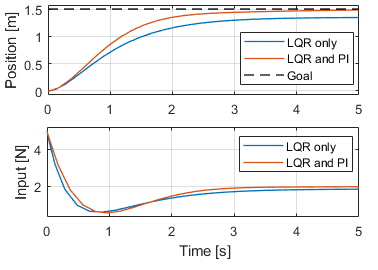
\includegraphics[width=0.5\textwidth]{MS.png}
	\caption{Comparison of LQR and LQR+PI controller. Position $x_1$ of the spring-mass system (top) and control input $u$ (bottom).}
	\label{fig:JanSM}
\end{figure} 

Note that only using the PI controller is not sufficient and would cause the system to become unstable.\\

For the pendulum, the iLQR algorithm converged to a cost of 156.70 after 52 iterations. The resulting trajectory is one initial swing to the left, followed by a complete upswing to the right. This trajectory seems reasonable, since reaching the goal with just a single swing is impossible due to the restrictions on the control input. Figure (\ref{fig:JanP1}) displays the trajectory that the algorithm found and the simulated trajectory with an added PID controller.
\begin{figure}[htp] 
	\centering
	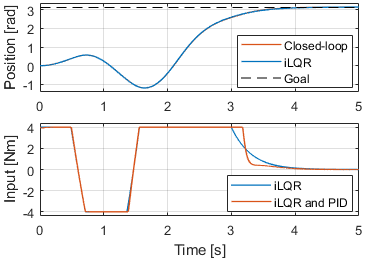
\includegraphics[width=0.5\textwidth]{P1.png}
	\caption{Comparison of iLQR result and closed-loop simulation. Angular position $x_1$ of the pendulum (top) and control input $u$ (bottom).}
	\label{fig:JanP1}
\end{figure} 

Both trajectories are almost identical, and there is only a small deviation in the control input at the end of the upswing (compare figure (\ref{fig:JanP1}) bottom at 3 seconds). However, this slight change is crucial to keep the pendulum in the upright position. Without the added PID controller, the system remains instable as shown in figure (\ref{fig:JanP2}), since iLQR is not a closed-loop controller.
\begin{figure}[htp] 
	\centering
	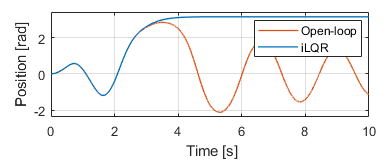
\includegraphics[width=0.5\textwidth]{P2.png}
	\caption{Comparison of iLQR result and open-loop simulation. Angular position $x_1$ of the pendulum.}
	\label{fig:JanP2}
\end{figure}\\

The MPC controller managed to stabilize the pendulum of the cart-pole in the upright position after 135 time steps or 2.7 seconds. Due to the input constraints, the car had to move left and right a few times to allow the pendulum to swing back and forth until it reached the upright position. The successful swing-up is presented in figure (\ref{fig:JanCP}). 
 \begin{figure}[htp] 
 	\centering
 	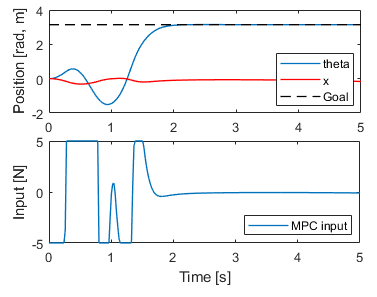
\includegraphics[width=0.5\textwidth]{CP.png}
 	\caption{The swing-up of the cart-pole system. Angular position $\theta=x_3$ of the pendulum and horizontal displacement $x=x_1$ of the car (top) and control input $u$ (bottom).}
 	\label{fig:JanCP}
 \end{figure}

Since MPC is a closed-loop control strategy, the system remained in the upright position after reaching it initially.

\section{COMPARISON AND DISCUSSION}
+TBD+

\section{CONCLUSION}
+TBD+



\begin{thebibliography}{99}

\bibitem{c1} G. O. Young, �Synthetic structure of industrial plastics (Book style with paper title and editor),� 	in Plastics, 2nd ed. vol. 3, J. Peters, Ed.  New York: McGraw-Hill, 1964, pp. 15�64.
\bibitem{c2} W.-K. Chen, Linear Networks and Systems (Book style).	Belmont, CA: Wadsworth, 1993, pp. 123�135.
\bibitem{c3} H. Poor, An Introduction to Signal Detection and Estimation.   New York: Springer-Verlag, 1985, ch. 4.
\bibitem{c4} B. Smith, �An approach to graphs of linear forms (Unpublished work style),� unpublished.
\bibitem{c5} E. H. Miller, �A note on reflector arrays (Periodical style�Accepted for publication),� IEEE Trans. Antennas Propagat., to be publised.
\bibitem{c6} J. Wang, �Fundamentals of erbium-doped fiber amplifiers arrays (Periodical style�Submitted for publication),� IEEE J. Quantum Electron., submitted for publication.
\bibitem{c7} C. J. Kaufman, Rocky Mountain Research Lab., Boulder, CO, private communication, May 1995.
\bibitem{c8} Y. Yorozu, M. Hirano, K. Oka, and Y. Tagawa, �Electron spectroscopy studies on magneto-optical media and plastic substrate interfaces(Translation Journals style),� IEEE Transl. J. Magn.Jpn., vol. 2, Aug. 1987, pp. 740�741 [Dig. 9th Annu. Conf. Magnetics Japan, 1982, p. 301].
\bibitem{c9} M. Young, The Techincal Writers Handbook.  Mill Valley, CA: University Science, 1989.
\bibitem{c10} J. U. Duncombe, �Infrared navigation�Part I: An assessment of feasibility (Periodical style),� IEEE Trans. Electron Devices, vol. ED-11, pp. 34�39, Jan. 1959.
\bibitem{c11} S. Chen, B. Mulgrew, and P. M. Grant, �A clustering technique for digital communications channel equalization using radial basis function networks,� IEEE Trans. Neural Networks, vol. 4, pp. 570�578, July 1993.
\bibitem{c12} R. W. Lucky, �Automatic equalization for digital communication,� Bell Syst. Tech. J., vol. 44, no. 4, pp. 547�588, Apr. 1965.
\bibitem{c13} S. P. Bingulac, �On the compatibility of adaptive controllers (Published Conference Proceedings style),� in Proc. 4th Annu. Allerton Conf. Circuits and Systems Theory, New York, 1994, pp. 8�16.
\bibitem{c14} G. R. Faulhaber, �Design of service systems with priority reservation,� in Conf. Rec. 1995 IEEE Int. Conf. Communications, pp. 3�8.
\bibitem{c15} W. D. Doyle, �Magnetization reversal in films with biaxial anisotropy,� in 1987 Proc. INTERMAG Conf., pp. 2.2-1�2.2-6.
\bibitem{c16} G. W. Juette and L. E. Zeffanella, �Radio noise currents n short sections on bundle conductors (Presented Conference Paper style),� presented at the IEEE Summer power Meeting, Dallas, TX, June 22�27, 1990, Paper 90 SM 690-0 PWRS.
\bibitem{c17} J. G. Kreifeldt, �An analysis of surface-detected EMG as an amplitude-modulated noise,� presented at the 1989 Int. Conf. Medicine and Biological Engineering, Chicago, IL.
\bibitem{c18} J. Williams, �Narrow-band analyzer (Thesis or Dissertation style),� Ph.D. dissertation, Dept. Elect. Eng., Harvard Univ., Cambridge, MA, 1993. 
\bibitem{c19} N. Kawasaki, �Parametric study of thermal and chemical nonequilibrium nozzle flow,� M.S. thesis, Dept. Electron. Eng., Osaka Univ., Osaka, Japan, 1993.
\bibitem{c20} J. P. Wilkinson, �Nonlinear resonant circuit devices (Patent style),� U.S. Patent 3 624 12, July 16, 1990. 






\end{thebibliography}




\end{document}
